\chapter{Circular Waveguide (2)}\label{lec:lec45}
Briefly  before  discussing the TE modes in circular waveguide, lets review the TM modes we treated in the previous lecture for the TM   mode in a circular waveguide whose dielectric has permeability given as $\mu$ and $\epsilon$ respectively, we know that the $E_z$ component exist and the boundary condition for the conducting surface in satisfied when $E_z(r=a)= 0$. We found that the solution of $E_z$ is $E_z = A_n J_n(hr)\cos(n\phi)$  where $h= \omega^2\mu + \gamma^2$  Then we observed that for the boundary condition certain modes exists which can be specified by two parameters n and p such that a specific TM mode is denoted by $TM_{np}$ where n shows how the amplitude varies in $\phi$ and also what order of the Bessel function in present while p shows which zero point (root) we goto to satisfy the boundary condition within the function $J_n(x)$. So  basically the modes are determined by how the amplitude varies in the $\phi$ direction and the number of lobes or wavelength we got in the r direction. We recall from  the last lecture that the n has to be an integer because the $\cos(n\phi)$ has to come back to the same value at $\phi=2\pi$ ie if we have gone a complete cycle, the amplitude should become the same otherwise we do not have a mode. So the two values which define a mode are n and p where  n like we said is the number of times we have variations in the $\phi$ direction and the order of the Bessel function and based on the order of the Bessel function p tells us which zero \textquoteleft0\textquoteright point we are considering to satisfy the boundary condition which in the number of lobes we would get in the $r$ direction. From our study of the Bessel functions we recall that only $J_o(hr)$ has an amplitude at hr = 0 and the rest $J_n(hr)$ function has amplitude which in zero at hr = 0 for $ n \ne 0$. Also we observed from the table that the lowest TM mode is the $TM_{01}$ mode where n = 0 and p = 1.  n = 0 implies there is no variation in the $\phi$ direction and p = 1 shows that there is only one peak or lobe in the r direction therefore $ha = 2.305$. So

$$ h = \frac{2.405}{a}$$ and $$f_c = \frac{2.405}{2\pi\sqrt{\mu\epsilon}} = \frac{0.383}{a\sqrt{\mu\epsilon}}\text{which is the cut-off frequency}$$

Now lets look at the colour 2D plot showing the electric field intensities for various TM modes.
\begin{figure}[h]
\centering
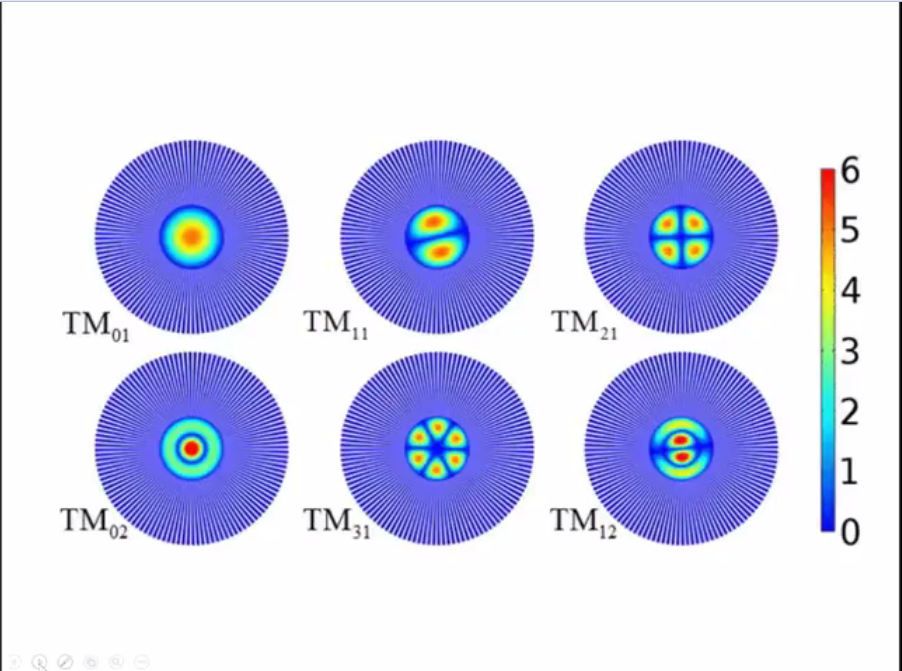
\includegraphics[width=0.9\linewidth]{\pathtoparttwo/graphics/colourplot}
\caption{2D colour plot of the TM modes.}
\label{fig:colourplot}
\end{figure}
$\underline{TM_{10} \ mode:}$ \ \ In the $\phi$ direction we observe that there is no variation and that in what $n=0$ means. Also if we consider the r direction, there is one lobe as shown in the plot. We can plot the field variation  in the r direction as shown below.
\begin{figure}[h]
\centering
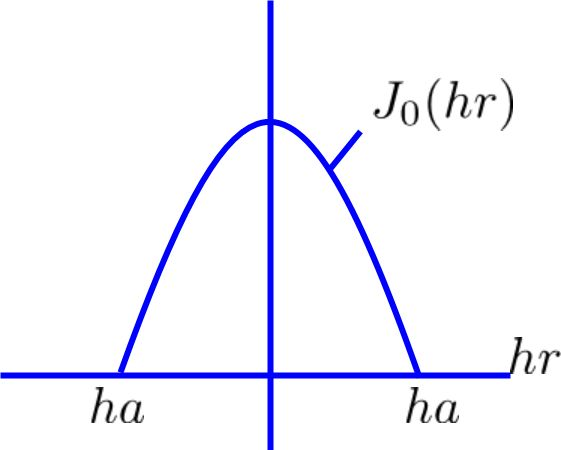
\includegraphics[width=0.5\linewidth]{\pathtoparttwo/graphics/m1}
\caption{}
\label{fig:m1}
\end{figure}
we observe that the field peaks at the centre and in zero at the boundary which is the same as the colour plot.
      
$\underline{TM_{02} \ mode:}$ \ \ Also we observe that there is no variation in the $\phi$ direction because if we draw a circle in the plot, we observe that there is no variation in the field intensity along the circle. This is what we should expect for $n =0$. Also, if we consider the r direction we observe that there are two peaks or lobes in that direction. However, these peaks have different magnitudes signified by the red and cyan color we see on the plot. Lets plot this variation as shown below;
\begin{figure}[h]
\centering
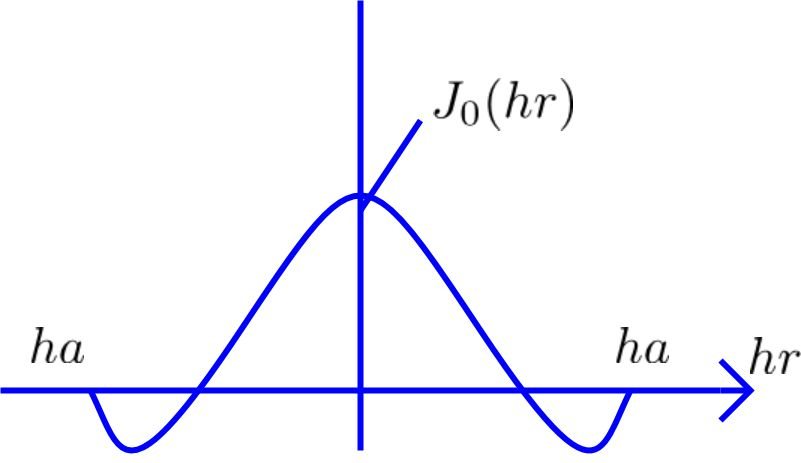
\includegraphics[width=0.7\linewidth]{./graphics/m2}
\caption{}
\label{fig:m2}
\end{figure}
It can be seen that the magnitude at the centre is the red color we see on the plot and the cyan color corresponds to the negative lobe with lesser amplitude, this observation is different to that of the rectangular waveguide where the amplitude of the  electric field is same for the lobes for instance if we consider the 3rd order mode in the y direction we will see a plot as shown below which shows that the amplitude stays the same.
\begin{figure}[h]
\centering
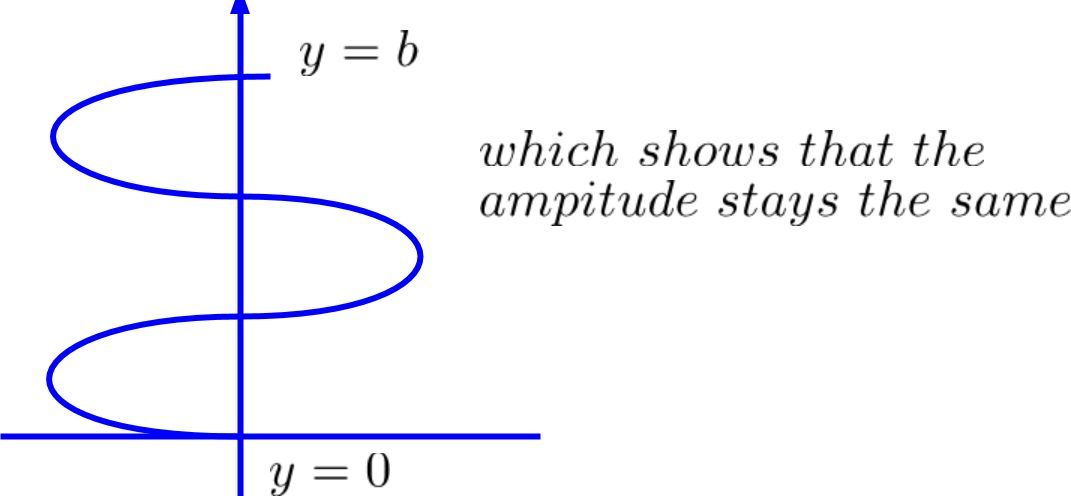
\includegraphics[width=0.5\linewidth]{\pathtoparttwo/graphics/m3}
\caption{}
\label{fig:m3}
\end{figure}
$\underline{TM_{11} \ mode:}$ \ As shown in the plot, these is one wavelength variation in the $\phi$ direction because the are two peaks (one is positive-maximum and the other is negative-minimum) and it also corresponds to the first order Bessel function $J_1(hr)$. For this mode $p =1$  so the boundary condition is at the first root of $J_1(hr).$ We recall that $J_1(hr)$ has a zero at $h_r =0$ (center of the waveguide) so there is no field  at the center indicated by the deep blue colour.

$\underline{TM_{21} \ mode:}$ \ \ for this mode $n=2$, so we expect two wavelength in the $\phi$ direction which corresponds to 4 peaks (2 maximum and 2 minimum) as shown in the plot. For  p = 1 there will be one peak in the r direction and it is plotted as shown below;
\begin{figure}[H]
\centering
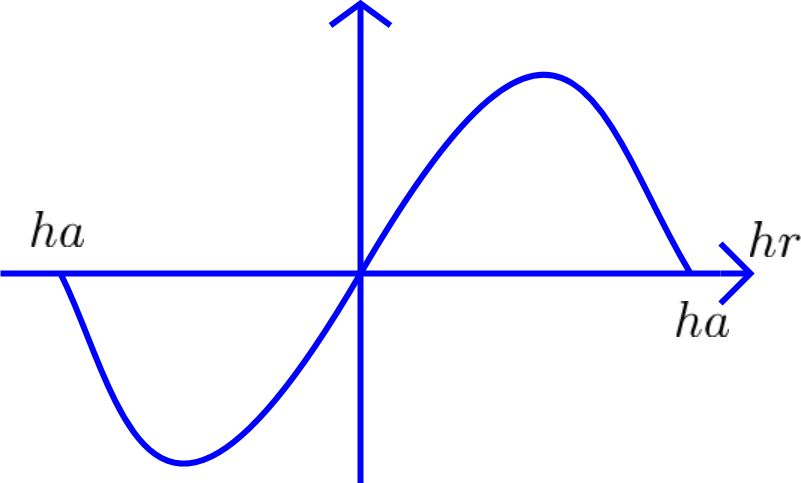
\includegraphics[width=0.5\linewidth]{\pathtoparttwo/graphics/m4}
\caption{}
\label{fig:m4}
\end{figure}

$\underline{TM_{31} \ mode:}$ \  \ For this mode n = 3 which equals 3 wavelength in the $\phi$ direction and it implies six peaks or lobes in that direction. Also for p = 1  it means we apply the boundary condition at the first zero point.

$\underline{TM_{12} \ mode:}$ \  \ Here n = 1 equals one wavelength in the $\phi$ direction corresponding to two lobes and p = 2 means we consider the second root of the   $J_1(hr)$ function. Therefore we will expect two lobes in the r direction as shown in the plot. Essentially n is the number of wavelength in the $\phi$  direction and p in the number of lobes in the r direction.
      
\section{TE modes}
 Now, let's take a look at the TE modes of  the circular waveguide. For this mode we need to study the derivative of the Bessel function. We recall 
$$ J_n(hr) = \sum_{k = 0}^{\infty}\dfrac{(-1)^k(hr)^{2k + n}}{k!(k+n)!2^{2k + n}} \quad \text{where n is an interger}$$
So the derivative of the Bessel function is given as $$ \dfrac{dJ_n(hr)}{dr} $$ and it is denoted by $J'_n(hr) $ and it is given as 
$$J'_n(hr) = \sum_{k = 0}^{\infty}\dfrac{(-1)^k h^{2k + n}(2k + n)r^{2k + n -1}}{k!(k+n)!2^{2k + n}} \ \ \ \text{by differetiating}$$		
$J_n(hr)$ with respect to r. Further simplification and substitution will give the relationship shown below 
$$ J'_n(hr) = \frac{1}{2}\bigg[J_{n-1}(hr) - J_{n + 1}(hr)\bigg] $$

For the circular waveguide we are only considering points where the boundary condition can be applied and as such the above relationship is not utilized here. However for dielectric waveguides like the optical fibre the relationship becomes useful for solving for the optical modes. So in terms of the circular waveguide we will work with the numerical values at which $J'_n(hr)$ goes to zero which is given in the table below;

\begin{table}[h]
\centering
\text{Zeros of $J'_n(hr)$}\\
\begin{tabular}{|c | c  c  c|}
\hline
\backslashbox{p}{n} & n=0 & n=1 & n=2 \\
\hline
1 & 3.832 & 1.841 & 3.054 \\
2 & 7.016 & 5.331 &6.706 \\
\hline
\end{tabular}
\end{table}

From the table, we observe that the lowest zero point is when n = 1 and p = 1 and this correspond to a $TE_{11}$ mode therefore the $TE_{11}$ mode is the lowest cut-off mode, followed by $TE_{21}$ and then $TE_{01}$ and so on.

For the TE mode we know that $E_z = 0$ and $H_z$ exists, so we will solve for the $H_z$   component which is given as;
$$H_z(r,\phi,z) = H_z(r,\phi)e^{-\gamma z}$$ So \begin{equation} \nabla^2 H_z(r,\phi) +  h^2 H_z(r,\phi) = 0\end{equation}
To solve this equation we repeat the procedure for the TM mode such that 
$$H_z(r,\phi)= R(r)\Phi(\phi)$$
Therefore equation we 1 becomes
$$ \frac{1}{r}\frac{\partial}{\partial r}\bigg(r\frac{\partial R\Phi}{\partial r}\bigg) + \frac{1}{r^2}\frac{\partial^2 R\Phi}{\partial \phi^2} + h^2\{R\Phi\} = 0$$
and it result in
\begin{equation}
\dfrac{d^2 R}{dr^2} + \frac{1}{r^2}\dfrac{dR}{dr} + \bigg(h^2 - \frac{n^2}{r^2}\bigg)R = 0
\end{equation}
and 
\begin{equation}
\dfrac{d^2\Phi}{d\phi^2} + n^2\Phi = 0
\end{equation}
The procedure is similar to the TM mode, the only difference is that we start with solving  the helmhottz wave equation for the magnetic field.
So the solution of the TE mode is 
$$ H_z(r,\phi) = A_nJ_n(hr)\cos(n\phi)$$
Now for this solution n has to be an integer. We can now solve for the other components. Recall;
$$ \overline{H}_\perp = \frac{j\omega t}{h^2}\nabla_\perp\times(E_z\hat{z}) - \frac{r}{h^2}\nabla_\perp H_z$$ and
$$\overline{E}_\perp = \frac{-j\omega \mu}{h^2}\nabla_\perp\times(H_z\hat{z}) - \frac{r}{h^2}\nabla_\perp E_z$$
for the TE mode $E_z = 0$ So 
\begin{align} 
\overline{H}_\perp = H_r \hat{r} + H_\phi \hat{\phi} &= \frac{-r}{h^2}\nabla_\perp H_z\\
&= \frac{-r}{h^2}\bigg\{ 
\hat{r}\frac{\partial H_z}{\partial} + \frac{\hat{\phi}}{r} \frac{\partial H_z}{\partial \phi}   
\bigg\}
\end{align}
Therefore
$$H_r = \frac{-r}{h^2}\frac{\partial H_z}{\partial r} =  \frac{-r}{h^2}A_nJ'_n(hr)\cos(n\phi)$$
For a lossless medium $ r =j\beta$

So 
$$H_r = \frac{-j\beta}{h^2}A_nJ'_n(hr)\cos(n\phi)$$
and
$$ H_\phi = \frac{-j\beta}{h^2}\frac{\partial H_z}{\partial \phi} =  \frac{-j\beta n}{h^2 r}A_nJ'_n(hr)\sin(n\phi)$$	 	
Also
\begin{dmath} 
\overline{E}_\perp = \frac{-j\omega\mu}{h^2}\nabla_\perp\times H_z\hat{z}
=\frac{-j\omega\mu}{h^2}
\bigg\{ 
\frac{1}{r}
\bigg|
\begin{matrix}
\hat{r} &  r\hat{\phi}  &  \hat{z}\\ 
\frac{\partial}{\partial r}  &  \frac{\partial}{\partial \phi}  &  0\\
0  &  0  &  H_z
\end{matrix}
\bigg| 
\bigg\}
\end{dmath}
\begin{dmath}
\overline{E}_\perp = E_r\hat{r} + E_\phi\hat{\phi} = \frac{j\omega\mu}{h^2} \bigg \{ \frac{1}{r}\frac{\partial H_z}{\partial \phi} - \frac{\partial H_z}{\partial r}\bigg\}
\end{dmath}
So 
$$ E_r = \frac{-j\omega\mu}{h^2 r}\frac{\partial H_z}{\partial \phi} = \frac{j\omega\mu n}{h^2 r}A_nJ_n(hr)\sin(n\phi)$$
And
$$ E_\phi = \frac{j\omega\mu}{h^2 }\frac{\partial H_z}{\partial \phi} = \frac{j\omega\mu }{h^2 }A_nJ'_n(hr)\cos(n\phi)$$
So the component are
\begin{align*}
H_r &= \frac{j\beta}{h^2 }A_nJ_n(hr)\cos(n\phi)\\ H_\phi &= \frac{j\beta}{h^2 r}A_nJ_n(hr)\sin(n\phi)\\
H_z &= A_nJ_n(hr)\cos(n\phi)\\
E_r &= \frac{j\omega\mu n}{h^2 r}A_nJ_n(hr)\sin(n\phi)\\
E_\phi &= \frac{j\omega\mu }{h^2 }A_nJ_n(hr)\cos(n\phi)\\
E_z & = 0
\end{align*}

We observe that $H_r$ depends on $\frac{\partial H_z}{\partial r},$ $H_\phi$ depends on $\frac{\partial H_z}{\partial \phi},$  $E_r$ depends on $\frac{\partial H_z}{\partial \phi}$ and $E_\phi$ depend on $\frac{\partial H_z}{\partial r}$. This shows that if we consider a field component in the z direction, we find the transverse component of this field as the derivative of the field with respect to the direction of each of the transverse component i.e $H_r \sim \frac{\partial H_z}{\partial r}$ and $H_\phi \sim \frac{\partial H_z}{\partial \phi}$  while we find transverse field component of the opposite of the opposite field from the derivative of the field with respect to the orthogonal direction to each of the transverse 	component of the opposite field i.e $H_r \sim \frac{\partial H_z}{\partial \phi}$ and $H_\phi \sim \frac{\partial H_z}{\partial r}$.     
For the TE mode we have the $E_\phi$ component  which is parallel to the conducting walls as shown below.
\begin{figure}[h]
\centering
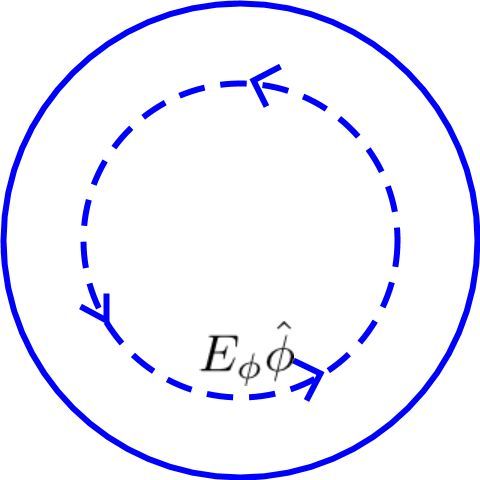
\includegraphics[width=0.5\linewidth]{./graphics/m5}
\label{fig:m5}
\end{figure}

We know that at the boundary the electric field has to go to zero so $E_\phi(r = 0)$ = 0 which implies $J'_n(ha) = 0$ for any specific TE mode. If we take a look at the table we discussed earlier we observe that the smallest value  of $ha$ for which we satisfy the boundary condition is when $ha= 1.841$ which is the TE mode with the lowest cut-off frequency. As we know n shows there is one wavelength variation in the $\phi$ direction and p = 1 shows that we are at  the first zero point of the $J'_1(hr)$ function.

So
$$(h)_{TE_{11}} = \frac{1.841}{a}$$
and the cut-off frequency of this mode is 
$$(f_c)_{TE_{11}} = \frac{(h)_{TE_{11}}}{2\pi\sqrt{\mu\epsilon}} = \frac{0.293}{a\sqrt{\mu\epsilon}}$$	
We recall that te lowest TE mode is the $TE_{01}$ mode which  to $(f_c)_{TE_{01}} = \frac{0.383}{a\sqrt{\mu\epsilon}}$ and if can be seen that the cut-off frequency of the $TE_{11}$ is less that that of the $TE_{01}$ mode. Hence the $TE_{11}$ mode is the dominant mode of the circular waveguide from the table we observe that the order of the mode are arranged from the lowest cut-off to the highest as \  $TE_{11}, \  TE_{21}, \ TE_{01}, \ TE_{12}, \ TE_{22} \ and \ TE_{02}$ which does not follows a nice order like the rectangular waveguide because of the derivative Bessel function terms.

\section{Attenuation in the circular waveguide}
 Lets discuss briefly, the attenuation in this mode. In terms of losses the behaviour will be similar to that of the parallel plane waveguide because the modes which have more energy close to the conducting wall will have more losses since these energies will excite current on field component parallel to the conducting walls will have more losses for the TE mode we have the $H_z$ and the $H_\phi$ component and for the TM mode we have the $H_\phi$ component only for most cases the losses drop as frequency increases and then increases, but there are unique mode present is any mode that is the $TE_{op}$ mode. For these modes the loss decreases monotonically as frequency increase which is shown below for the case of $TE_{01}$ mode 
\begin{figure}[h]
\centering
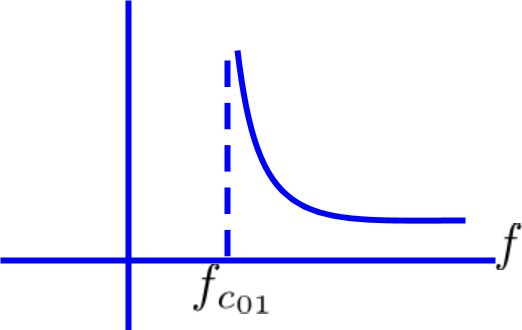
\includegraphics[width=.5\linewidth]{\pathtoparttwo/graphics/m6}
\caption{}
\label{fig:m6}
\end{figure}

So there is no minimum with respect to frequency. The $TE_{op}$ mode is unique in this sense because no other mode whether it is circuit or rectangular waveguide, has this behaviour this end our discussion on circular waveguide.